% !TEX root = ../notes_template.tex
\chapter{Oral Microbiome}\label{chp:oral_microbiome}

\minitoc

\section{Introduction}

It is the second large microbiome in the human body, after the gut, with more easy access. Presents spatially organized 
biofilms \cite{Welch2020,Wilbert2020}, which derives in the site-specialist hypothesis that predicts that most microbes 
in the human oral cavity have a primary habitat type within the mouth where they are most abundant. 

\begin{definition}[Habitat]
Refers to externalities such as the physical space and chemical environment that allow and organism to exist, 
including contributions from other members of the microbial community.    
\end{definition}
\begin{definition}[Niche]
Refers to the activity of an organism and the functional role that each member plays in the community. Interactions of 
the member both with one another and with the habitat drive the emergent organization of the community as a whole.
\end{definition}

Importance of the spatial organization in various aspects of the human microbial ecology \cite{Proctor2017}.  

\section{Major oral habitats}
The mouth is an open system. Microbes are breathed with the air, ingested with the food, or acquired through close 
contact (animals, humans, or surroundings). 

Although the millions of bacterial species on the planet discovered so far (and other millions to remain discovered), 
it is believed that only approximately 760 are primary residents, rather than transients in the mouth, according to the 
Human Oral Microbiome Database \cite{Escapa2018} \marginpar[left]{In my opinion this number is not informative, as don't 
take into account any prevalance among population, including rare and probably transient species}.
\begin{itemize}
    \item Supragingival plaque
    \item Subgingival plaque 
    \item Keratinized gingiva 
    \item Hard palate 
    \item Buccal mucosa 
    \item Throat 
    \item Palatine tonsils 
    \item Tongue dorsum 
\end{itemize}

Each of these sites is not monolithic, rather sheltered or exposed to different environmental conditions: 
\begin{itemize}
    \item Crowns of teeth abundant of oxygen.
    \item Tooth surface in the gingival crevice anorexic environment bathed in gingival crevicular fluid, protein-rich 
    exudate from the gingival tissues. 
    \item Saliva film thinnest at the roof of the mouth in contrast with the saliva pools at the floor. 
    \item Similarly, relative proximity to salivary glands influences the composition and rate of flow of saliva. 
\end{itemize}

Although saliva is not a habitat per se, there are evidence that microbes found within the saliva are not abundant at 
any of the other sampled sites, suggesting additional unique micro-habitats elsewhere in the mouth. 

\section{Selective force within the mouth}
\begin{itemize}[Flow and adhesion]
    \item Salivary flow imposes a selective requirement for adherence: microbes can persist in exposed locations in the 
    mouth only if they are adhered to an underlying substrate or to other microbes that are able to adhere to the substrate. 
    \item In addition, salivary flow also requires closely proximity for microbial interactions, as microbial metabolites 
    are constantly washed. Interestingly,  
    \item In response to selective pressures, oral microbes developed highly specific adhesin-receptor interactions, 
    which form the basis for cohesion or coaggregation phenomenon. 
\end{itemize}

\begin{itemize}[Shedding and colonization]
    \item Dynamics of shedding of the underlying substrate and re-colonization back to the substrate.
    \item Overall thickness of the microbial biofilm is influenced by the rate of shedding. Exposed areas: enamel teeth 
    surface, mucosal surfaces. Factors: oral hygiene, abrasion by chewing food. 
    \item Colonization of fresh substates after shedding and abrasion. This colonization is dependent on both microbial 
    and host sources, e.g. colonizing streptococci bind to cysteine repeat domains within glycoproteins or sialic acid of 
    mucin in the enamel pellicle, whereas adherence of specific bacteria to the mucosa could be mediated in part by the secretory 
    immunoglobulin A.
\end{itemize}

\begin{itemize}[Host and microbe]
    \item Saliva flow and immune surveillance are properties of the host that reduce the microbial load. 
    \item Saliva is also a vehicle for positive selection of microbes cause mucins and nutrients such as lactate, 
    bicarbonate, nitrate, and vitamins are actively secreted into saliva \cite{Carperter2020}.
\end{itemize}  

\begin{tcolorbox}[
    title=Saliva,
    title filled=false,
    colback=blue!5!white,
    colframe=blue!75!black]
    Saliva is formed by an active process of ion secretion into the lumen of the gland, creating an osmotic gradient which 
    draws water through from the interstitial space. 

    \begin{itemize}
        \item Most ions and metabolites are transported by specific channels into saliva. 
        \item Proteins are synthesized in the glands and added mostly by a separate mechanism of storage granule release
        dependant on cyclic adenosine monophosphate (AMP) signaling:
        \begin{itemize}
            \item Saliva directly from the duct: few serum proteins.
            \item Whole mouth saliva: high amount of serum proteins derived from a serum transudate leaking around teeth 
            (via gingival crevicular fluid).
        \end{itemize}
        \item Urea concentrations  parotid saliva > whole mouth saliva/plasma -> active transport of urea into parotid 
        saliva + use by bacteria.
        \begin{itemize}
            \item Urea is the most non-protein nutrient in saliva, used by \textit{Streptococcus salivaris}, 
            \textit{Actinomyces naeslundii}, \textit{Haemophilus} by their expression of urease 
            (urea -> ammonia + CO2 or urea -> ammonium carbamate -> Formate). Urease is not present in mammalian cells. 
            Indeed, this reaction is so reliable that it is the basis of the urea breath test for \textit{Helicobacter pylori} 
            infections of the gut \autoref{fig:urea_test}. 
        \end{itemize}
        \item Low levels of sugars/carbohydrates in absence of food. Bacteria presumably rapidly utilize them via the 
        Embden Meyerhof Parnas (EMP) pathway \autoref{fig:saliva_content}.
        \begin{itemize}
            \item Carbohydrates sources from food are still detectable after 20min, but usually clear in the mouth after 
            1h. -> CH not may fuel source for commensal bacteria. 
            \item Proteins as main fuel source by proteolytic degradation of salivary proteins. 
            \item The Arginine Deiminase System (ADS) hydrolyses arginine to create citrulline and ammonia; the ammonia 
            is beneficial to the host by neutralizing lactic acid in carious lesions. This pathway has become prominent 
            as some dental products now contain arginine as an additive. 
            \item CH linked to proteins (glycoproteins) can also be used by sialidases action and other glycosidases 
            (glycolytic EMP pathway = glucose -> pyruvate). Here importance of bacteria cooperation in biofilms as no 
            single bacterium contains all the necessary enzymes involved in the EMP pathway. 
        \end{itemize}
        \begin{itemize}[Nitrate]
            \item Actively transported from the blood system by the salivary glands via the sialin transporter and delivered into the saliva. 
            \item Bacteria including Rothia and Veillonella nitrate -> nitrite (+ stomach acid) -> NO. 
            \item Cor(Salivary nitrate, lowered caries risk).
            \item Altered microbiome by long-term nitrate supplementation -> utilization.
        \end{itemize}
        \begin{itemize}[Lactate]
            \item Connected to a high diversity in the mouth. Lactate consumers present in multi-species biolfilms -> syntrophy. 
            \item Actively secreted by saliva.
        \end{itemize}
        \begin{itemize}[Bicarbonate]
            \item Actively secreted by salivary mucin-secreting sublingual and minor glands.
            \item Consumers and producers such as Streptococcus anginosus and Porphyromonas gingivalis, respectively.
        \end{itemize}
        \begin{itemize}[Limitation of other nutrients availability]
            \item Chelation of iron by binding to iron-free lactoferrin. 
            \item Cobalamin (B12 vitamin). Not transport from serum to saliva + transcobalamin 
            (vitamin-binding proteins) -> Prevents use by bacteria such as P. gingivalis. 
        \end{itemize}
    \end{itemize}

    \begin{figure}[!ht]
        \centering
        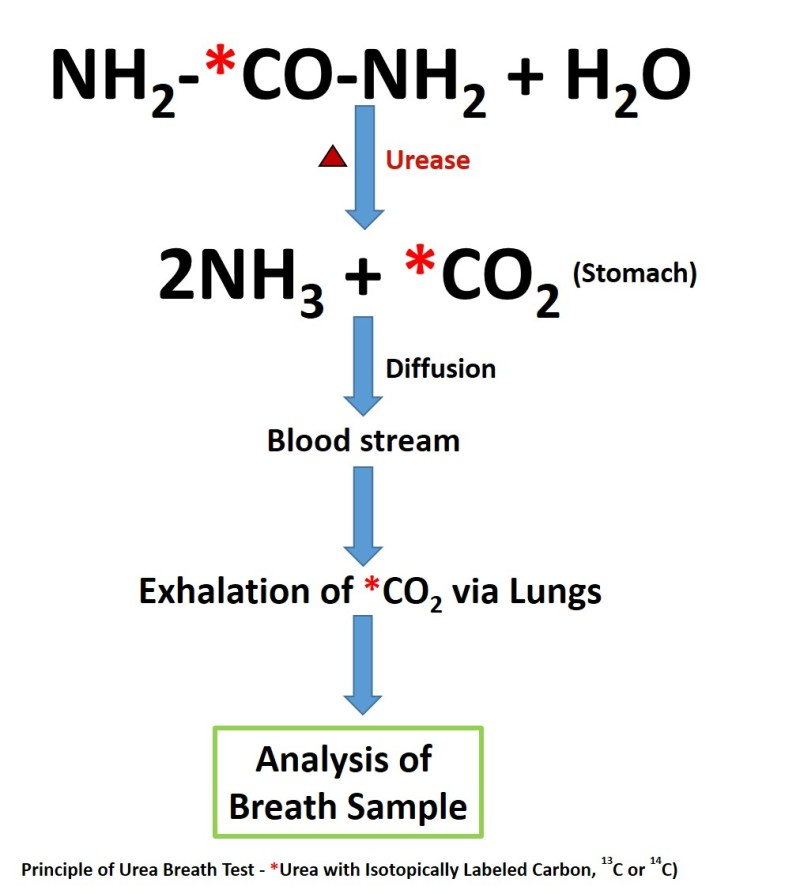
\includegraphics[width=1\linewidth]{./figure/urea_test.jpg}
        \caption{Urea breath test pathway. Borrowed from  Sankararaman S, Moosavi L. Urea Breath Test. [Updated 2024 Feb 23]. 
        In: StatPearls [Internet]. Treasure Island (FL): StatPearls Publishing; 2024 Jan-. Available 
        from: https://www.ncbi.nlm.nih.gov/books/NBK542286/}
        \label{fig:urea_test}
    \end{figure}
    \begin{figure}[!ht]
        \centering
        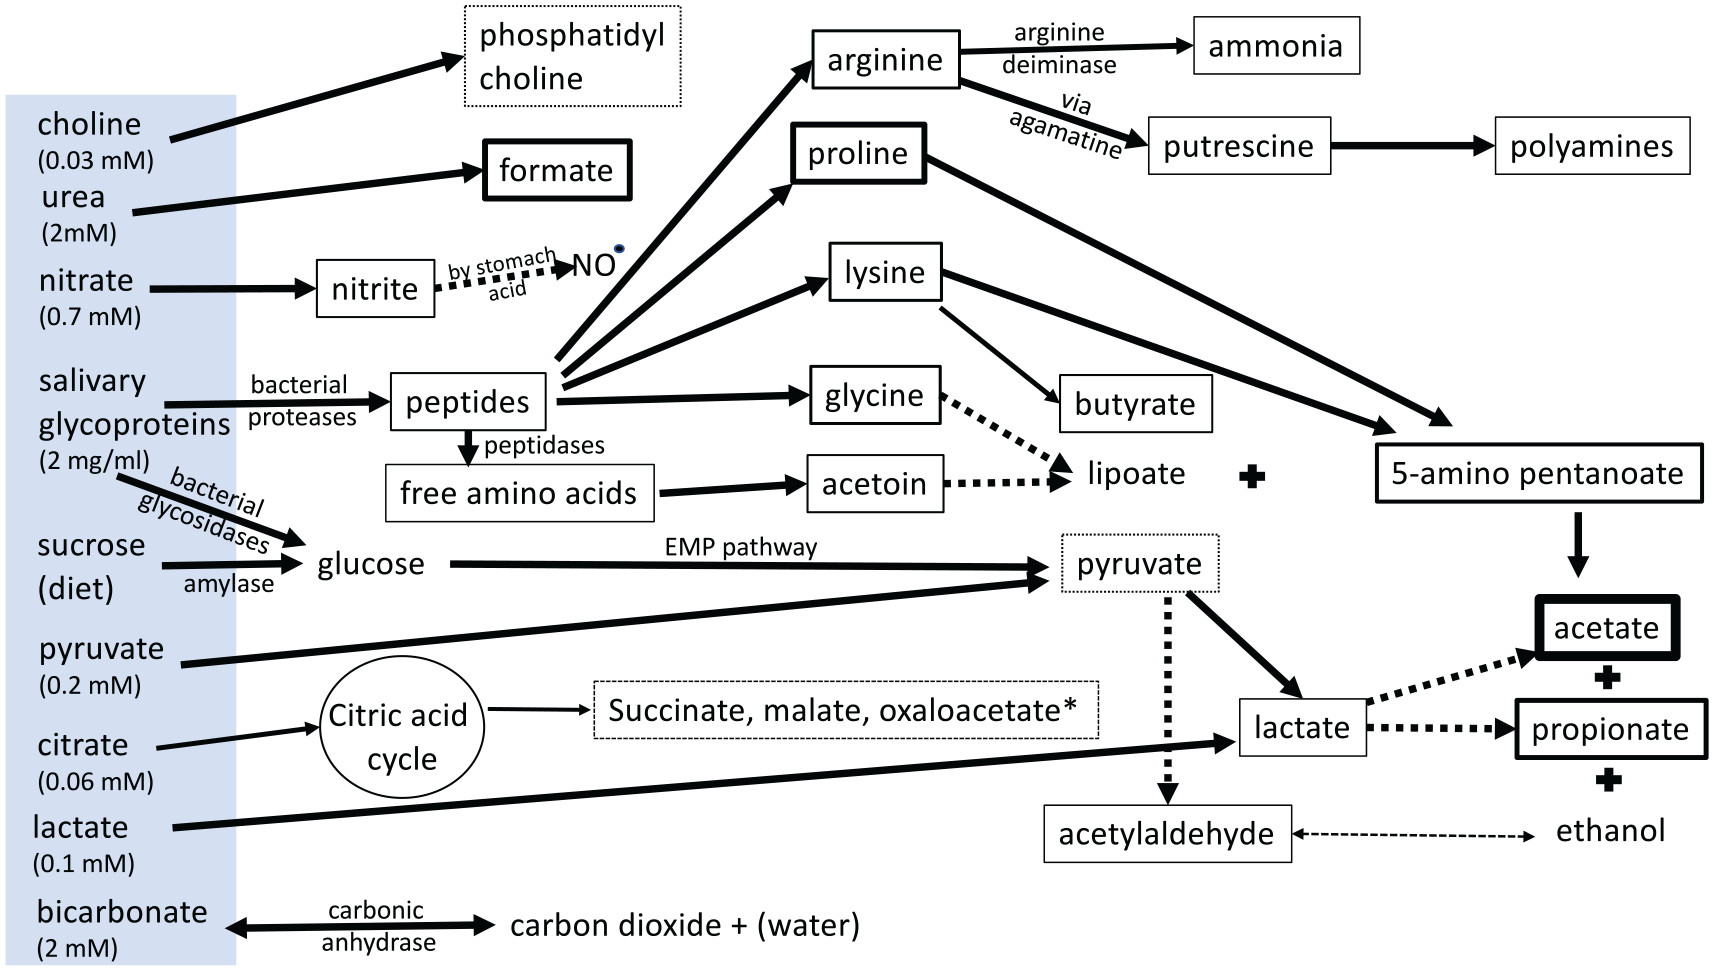
\includegraphics[width=1\linewidth]{./figure/saliva_content.jpeg}
        \caption{The main bacterial substrates (blue box) and detected metabolites (indicated by boxes) in whole mouth saliva. 
        The thickness of arrows and boxes indicates relative abundance, dotted lines indicate possible connections. 
        Under resting conditions between meals, the products of the citric acid cycle (indicated by *) are largely undetectable. 
        Most metabolites indicate the breakdown of salivary glycoproteins as the main nutrient source, the amino acids 
        yielding acetate and propionate, the N- and O-linked glycans leading to pyruvate via the Embden Meyerhof Parnas (EMP) pathway. 
        Borrowed from \citetitle{Carperter2020} \cite{Carperter2020}}
        \label{fig:saliva_content}
    \end{figure}
\end{tcolorbox}